\documentclass[../main.tex]{subfiles}
\graphicspath{{\subfix{../images/}}} % Images path

\begin{document}

\section{Appendix}\label{appendix}

\subsection{Confusion Matrices}\label{app:confusion-matrices}

Here the confusion matrices for all the classifiers are reported. These matrices refers to the case in which features have been extracted by a SIFT descriptor from keypoints sampled on a dense grid on the images and the input representation is the normalized histograms of visual words. This has been done to maintain the results consistent with the ones obtained using the spatial pyramid matching approach and to be able to compare the performances of the different classifiers. However, similar matrices can be computed in the other cases as well.\\

\begin{figure}[htb]
  \centering
  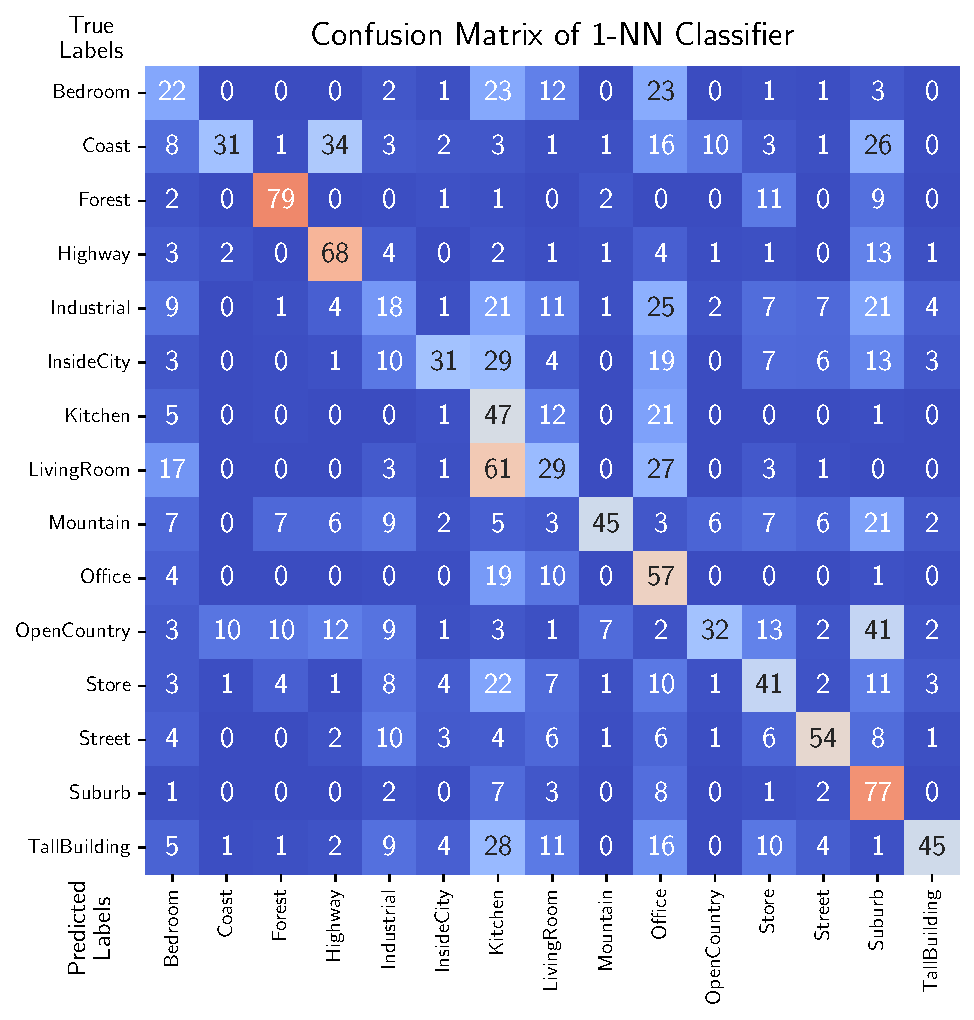
\includegraphics[width=0.8\textwidth]{1nn_confusion_matrix.pdf}
  \caption{Confusion matrix for the 1-NN classifier.}\label{fig:confusion-matrix-1nn}
\end{figure}

\begin{figure}[htb]
  \centering
  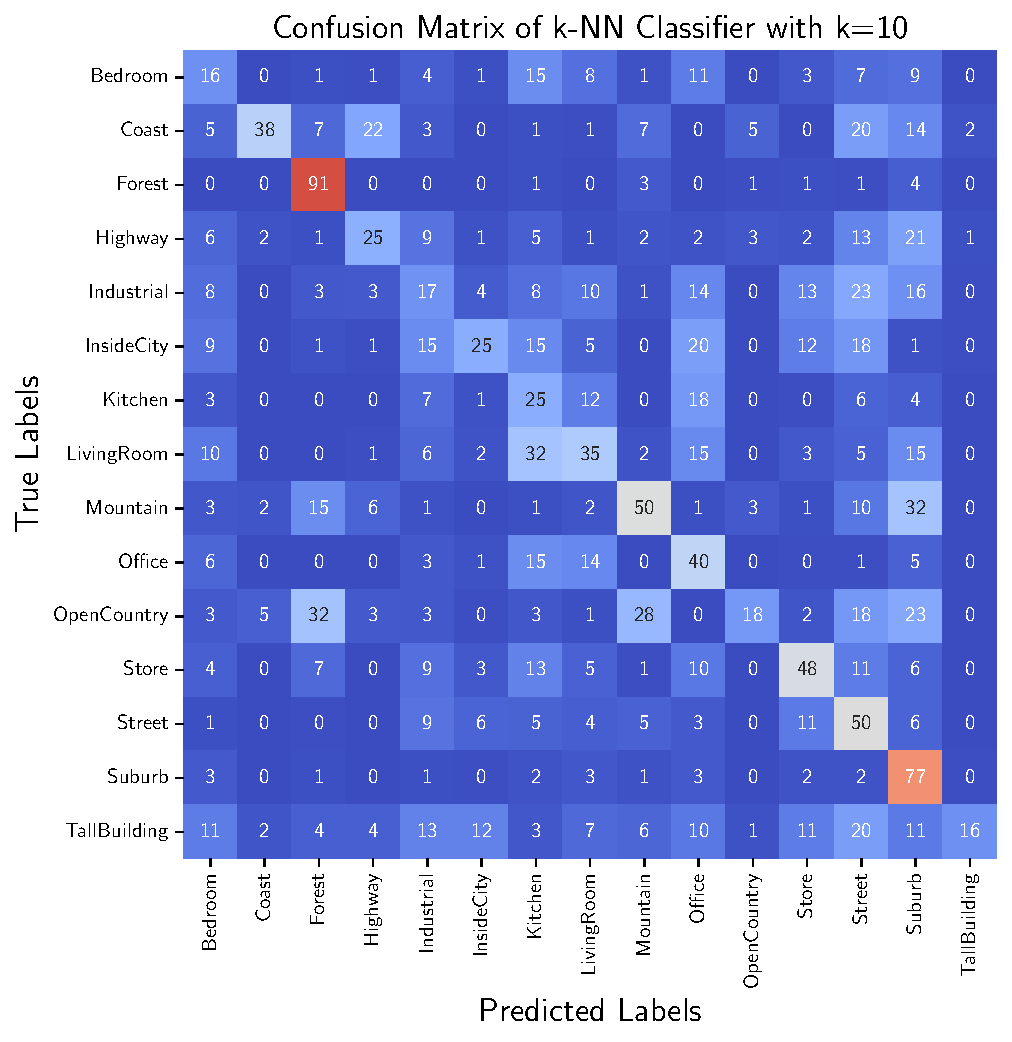
\includegraphics[width=0.8\textwidth]{knn_confusion_matrix.pdf}
  \caption{Confusion matrix for the k-NN classifier with $k = 20$.}\label{fig:confusion-matrix-knn}
\end{figure}

\begin{figure}[htb]
  \centering
  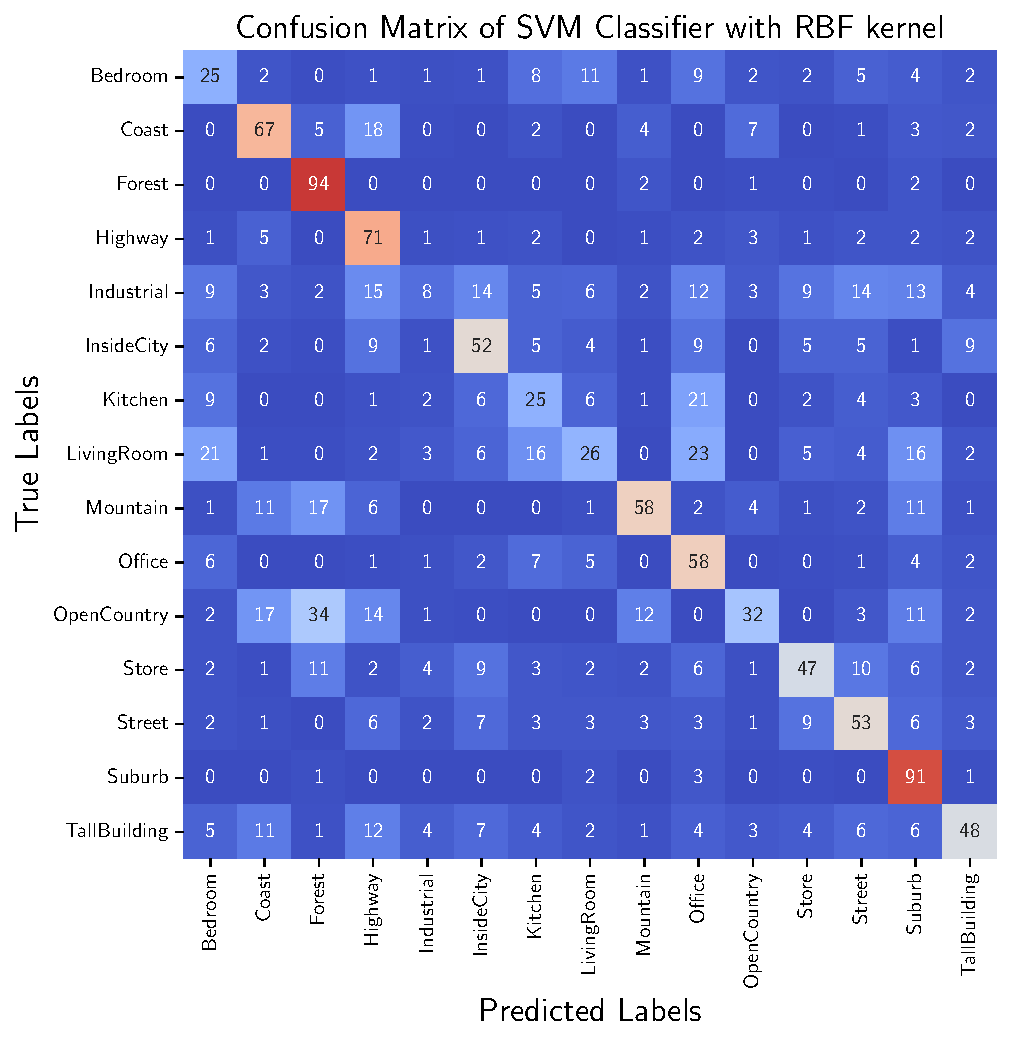
\includegraphics[width=0.8\textwidth]{svm_rbf_confusion_matrix.pdf}
  \caption{Confusion matrix for the SVM classifier with RBF kernel.}\label{fig:confusion-matrix-rbf}
\end{figure}

\begin{figure}[htb]
  \centering
  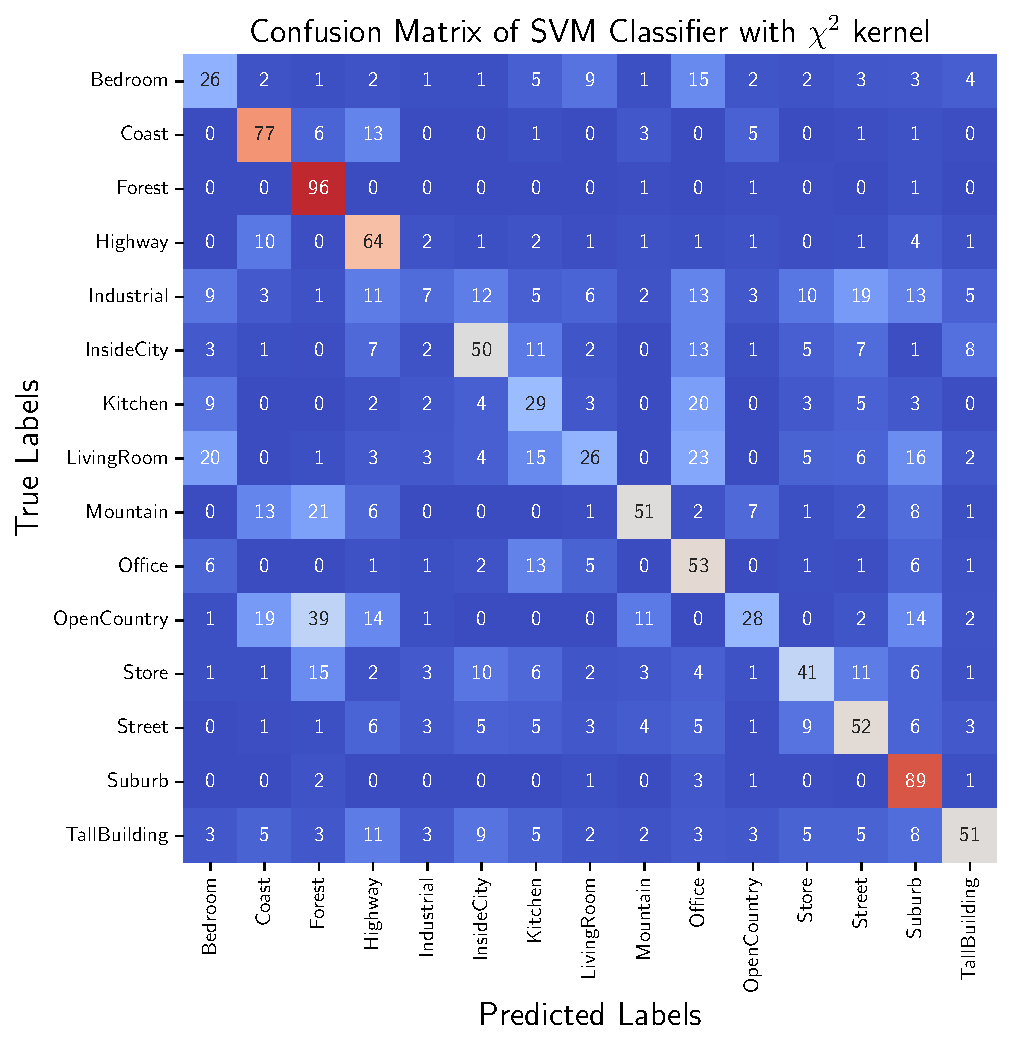
\includegraphics[width=0.8\textwidth]{svm_chi2_confusion_matrix.pdf}
  \caption{Confusion matrix for the SVM classifier with $\chi^2$ kernel.}\label{fig:confusion-matrix-chi2}
\end{figure}

\begin{figure}[htb]
  \centering
  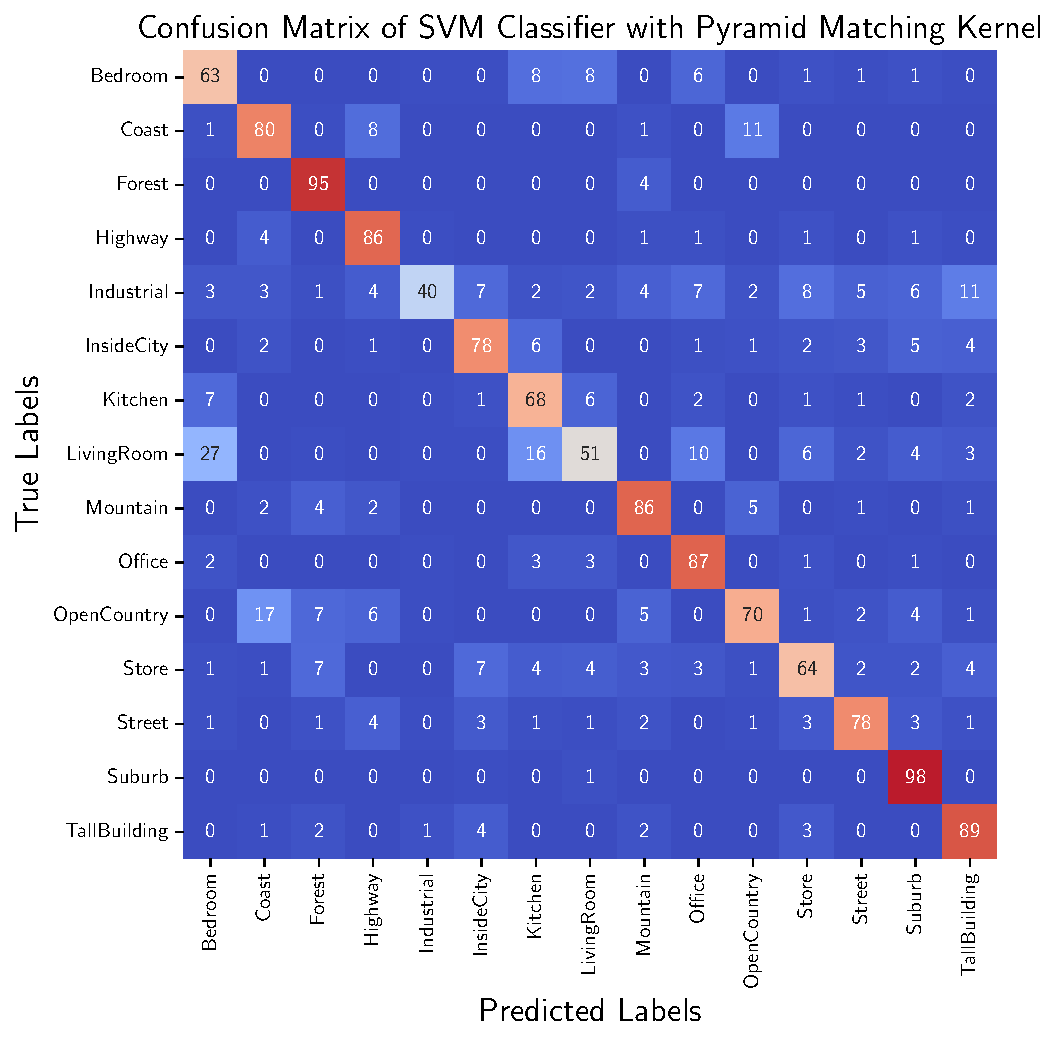
\includegraphics[width=0.8\textwidth]{svm_pmk_confusion_matrix.pdf}
  \caption{Confusion matrix for the SVM classifier with spatial pyramid matching kernel.}\label{fig:confusion-matrix-pmk}
\end{figure}

\end{document}


